% Complete Section 7.6, original PDF 100-101 / printed 90-91.
% block: whitney-forms-de-rham-heading page:100 type:section
\subsection{{Whitney 形式 $\mathcal P_1^-\Lambda^k$ 与 de Rham 定理}}\label{sec:whitney-forms-de-rham}

% block: whitney-forms-geometric-dofs page:100 type:ordinary-paragraph
{最低次修剪多项式有限元空间 $\mathcal P_1^-\Lambda^k(\mathcal T_h)$ 是 $H\Lambda^k(\Omega)$ 的子空间. 它的元素称为\emph{Whitney $k$-形式}. 其形函数 $\mathcal P_1^-\Lambda^k=\mathcal P_0\Lambda^k+\kappa\mathcal P_0\Lambda^{k+1}$ 构成线性多项式 $k$-形式的完全空间 $\mathcal P_1\Lambda^k$ 的子空间 (当 $k>0$ 时为真子空间). Figure~\ref{fig:whitney-form-dofs} 展示了表示三维中四个空间 $\mathcal P_1^-\Lambda^k$, $0\leq k\leq3$ 的单元图. 每幅单元图画出一个单纯形, 在面上放置符号, 标明该面上的各个自由度. 注意, Whitney 形式的自由度具有很强的几何性: 对 Whitney $k$-形式, 每个 $k$ 维子单纯形上恰有一个自由度, 即迹在该面上的积分, 而其他维数的面上没有自由度. 事实上, 这些空间独立于有限元, 已在 Hassler Whitney 于 1957 年出版的著作 \BookCite{70} 中出现.}

% block: whitney-form-complex pages:100,101 type:ordinary-paragraph
{如前所见, Whitney 形式组装成一个上链复形:}
\begin{equation}\label{eq:whitney-form-complex}
0\to\mathcal P_1^-\Lambda^0(\mathcal T_h)\xrightarrow{d}\mathcal P_1^-\Lambda^1(\mathcal T_h)\xrightarrow{d}\cdots\xrightarrow{d}\mathcal P_1^-\Lambda^1(\mathcal T_h)\to0,
\end{equation}
{它是与剖分 $\mathcal T_h$ 关联的 $L^2$ de Rham 复形的离散子复形. 还记得, $\mathcal P_1^-\Lambda^k(\mathcal T_h)$ 中的 Whitney 形式在 $k$ 维面上有良定义的迹. 事实上, 在 $k$ 维面上的迹是单值的, 这本来就是该空间定义的一部分.}
\footnote{{事实上, Whitney $k$-形式在 $k$ 维面 $f$ 上的迹是常 $k$-形式, 因为它属于 $\mathcal P_1^-\Lambda^k(f)$, 而在 $k$ 维区域上, $\mathcal P_1^-\Lambda^k$ 化为 $\mathcal P_0\Lambda^k$.}}
{因此, 将微分 $k$-形式映为 $k$-上链的 de Rham 映射 $F^k$, 在 Whitney 形式上是良定义的:}
\[
F^k\phi(g)=\int_g\operatorname{tr}_g\phi,\qquad\phi\in\mathcal P_1^-\Lambda^k(\mathcal T_h),\quad g\in\Delta_k(\mathcal T_h).
\]

% block: whitney-form-dofs-figure page:101 type:figure
\begin{figure}[htbp]\centering
\includegraphics[page=101,trim=112bp 572bp 85bp 62bp,clip,width=.90\linewidth]{../input/source/Finite Element Exterior Calculus.pdf}
\caption{{三维中 Whitney 形式的自由度.}}\label{fig:whitney-form-dofs}
\end{figure}

% block: whitney-simplicial-cochain-isomorphism page:101 type:ordinary-paragraph
{注意, 值 $F^k\phi(g)$ 正是 $\phi$ 的自由度: 它们可以任意指定, 并唯一确定 $\phi$ 的一个元素. 换言之, de Rham 映射 $F^k$ 定义了从 Whitney $k$-形式空间 $\mathcal P_1^-\Lambda^k(\mathcal T_h)$ 到单纯 $k$-上链空间 $C^k(\mathcal T_h)$ 的同构. 当 $k$ 变化时, 这些同构构成上链映射, 这在 Chapter~\ref{chap:homological-algebra} 中已经见过. 简言之, \emph{de Rham 映射是 Whitney 形式复形与单纯上链复形之间的上链同构}.}

% block: whitney-proof-of-de-rham-theorem page:101 type:ordinary-paragraph
{可以用 Whitney 形式证明在 Chapter~\ref{chap:homological-algebra} 末尾陈述过的 de Rham 定理的一个版本. Whitney 形式复形 \eqref{eq:whitney-form-complex} 的上同调当然同构于单纯上同调. 事实上, 同构的不仅是其上同调, 而且是复形本身. 现在考虑从 $L^2$ de Rham 复形到 Whitney 复形的有界上链投影, 我们知道它存在. 由 Theorem~\ref{thm:discrete-cohomology-isomorphism}, 只要逼近性质 \eqref{eq:harmonic-projection-strict-error} 成立, 该投影就诱导 de Rham 上同调到 Whitney 复形上同调的同构. 当网格尺寸充分小时, 该性质当然成立, 而网格总能通过加密变得足够细. 事实上, 它对任意网格都成立, 因为容易证明单纯上同调在加密下保持不变.}

% block: de-rham-cohomology-isomorphism-qualification page:101 type:remark
\Needspace{8\baselineskip}
\begin{Remark}\label{rem:de-rham-cohomology-isomorphism}
{已经证明, $L^2$ de Rham 上同调同构于单纯上同调. De Rham 定理更常用光滑 de Rham 上同调来陈述, 但这并非重大区别, 因为光滑与 $L^2$ de Rham 上同调本身就通过包含映射同构, 这本质上源于椭圆正则性. 见 [\BookNumber{24}, Theorem 2.12]. 更重要的区别在于, 这里给出的同构由磨光投影算子 (有界上链投影) 诱导, 而非由 de Rham 映射诱导, 后者并不定义在整个 $H\Lambda^k$ 空间上.}
\end{Remark}
